\chapter{Planejamento da avaliação}

    Faz parte do escopo da avaliação, a análise, sob a ótica de IHC, de todos os requisitos funcionais e os
    requisitos não-funcionais, analisando os princípios e metas de usabilidade desejados para o produto e as
    metas decorrentes da experiência do usuário.

    A avaliação tem por objetivos avaliar a aceitação da tecnologia pelo usuário, validar ideias e designs alternativos e buscar 
    por problemas na interface e na interação.
  
    A análise dos \textit{storyboards} e do protótipo de papel fornecem insumos para identificar problemas na interação e na interface,
    sendo a primeira avaliação a ser feita no projeto, com caráter inspecionista.
    
    Avaliações bem planejadas seguem metas claras e perguntas adequadas Brasili \textit{et al.} (1994 \textit{apud} \cite{preece}).
    Para orientar as nossas avaliações, utilizaremos o \textit{framework} DECIDE. Este \textit{framework} nos oferece uma lista
    de checagem para orientar nas avaliações pessoas com pouca experiência, que é o caso da equipe de avaliadores. Para
    a orientação da avaliação do projeto foi utilizado o \textit{framework} apresentado por \citeauthor{preece} (\citeyear{preece}),
    que conta com os seguintes tópicos para a avaliação:
    
    \begin{itemize}
       \item Determinar as metas que a avaliação irá abordar.
       \subitem Segundo \cite{preece}, as metas escolhidas devem guiar a avaliação, ou seja, o resultado da avaliação deve propor melhorias 
       que atingem estas metas estabelecidas para que haja a evolução do protótipo. As metas que se deseja alcançar para a avaliação do 
       aplicativo \textit{MyPush} estão descritas na seção 4 deste documento.
    \end{itemize}
    
    \begin{itemize}
    
       \item Explorar as questões específicas a serem respondidas.
       \subitem Para que se alcance as metas de avaliação definidas, deve-se escolher questões cujas respostas satisfaçam à elas. 
       O item 7.1.7 deste documento traz os questionários que foram definidos para que as metas no aplicativo \textit{MyPush} sejam alcançadas.
       
    \end{itemize}
    
    \begin{itemize}
    
       \item Identificar questões práticas que devem ser abordadas.
       \subitem Algumas questões práticas devem ser consideradas antes do início da avaliação. Deve ser feito uma seleção adequada dos usuários 
       que avaliarão a ferramenta, pois estes precisam representar a população pelo qual a aplicação será direcionada. Deve-se considerar quais 
       equipamentos a equipe irá utilizar para a avaliação: Câmeras, mesa, cadeira, caneta, papel, etc. Deve se considerar também se a equipe
       de avaliação possui conhecimento necessário para realizar a avaliação. Estes membros devem estar totalmente por dentrode todas as 
       funcionalidades que o protótipo possui. 
       
    \end{itemize}
       
    \begin{itemize}
    
       \item Decidir como lidar com as questões éticas.
       \subitem A equipe responsável pela avaliação da ferramenta deve se atentar sobre as questões éticas no processo da avaliação. Deve se manter a 
       privacidade das pessoas que farão parte da avaliação da ferramenta e isto deve ficar claro à eles antes da avaliação, quando são convidados a 
       participar da mesma através do termo de consentimento. Seus registros pessoais ficar ser confidenciais. Os usuários devem ser informados sobre 
       o tipo de registro das avaliações: filmagem, foto, etc.
       
    \end{itemize}
       
    \begin{itemize}
    
       \item Avaliar, interpretar e apresentar os dados.
       \subitem Os dados recolhidos nas avaliações do protótipo serão analisados, interpretados e, caso a equipe julgue necessário, considerados no desenvolvimento da aplicação.
   
   \end{itemize}
   
   \section{Termo de consentimento}
   
	O termo de consentimento é um termo a qual o usuário que será avaliado deve assinar antes da avaliação, 
	caso ele queira participar do processo de avaliação. Este termo assegura à equipe de avaliação que o usuário
	está ciente dos objetivos da avaliação e interessado em participar da mesma. O termo de consentimento utilizado
	para este trabalho segue o modelo feito por \citeauthor{termoconsentimento} (\citeyear{termoconsentimento}) e
	se encontra em anexo junto a dois termos preenchidos por usuários que participaram
	da primeira iteração de avaliação.

  \section{Estudos dos questionários}
    
    Os seguintes questionários foram analisados para a definição dos que seriam utilizados no projeto.
    
    \subsection{\textit{Software Usability Measurement Inventory} - SUMI}
      
      \nocite{summi}
      SUMI é um rigoroso questionário que tem a finalidade de medir a qualidade de um software do ponto de vista do usuário.
      Ele é composto por 50 questões e possui três níveis de resposta: Concordo, Indeciso e Não Concordo. O SUMI seria utilizado
      para avaliar a qualidade dos requisitos do \textit{MyPush} pelos usuários. Essas avaliações possibilitariam que o aplicativo fosse
      melhorado a cada versão.
      
    \subsection{\textit{Website Analysis MeasureMent Inventory} - WAMMI}
      
      \nocite{wammi}
      O \textit{Website Analysis MeasureMent Inventory} (WAMMI) é um serviço analítico para a \textit{web} que mede e analisa a experiência do
      usuário em um \textit{website}, baseado na reação dos visitantes. Essa reação dos visitantes é medida com base na comparação das
      expectativas do usuário com o que realmente foi encontrado no \textit{site}, por meio de um questionário de 20 questões que pode
      ser expandido com algumas questões adicionais. A Figura ~\ref{wammi_questions} ilustra um exemplo dos itens do questionário WAMMI.
      
      \begin{figure}[!htpb]
	\centering
	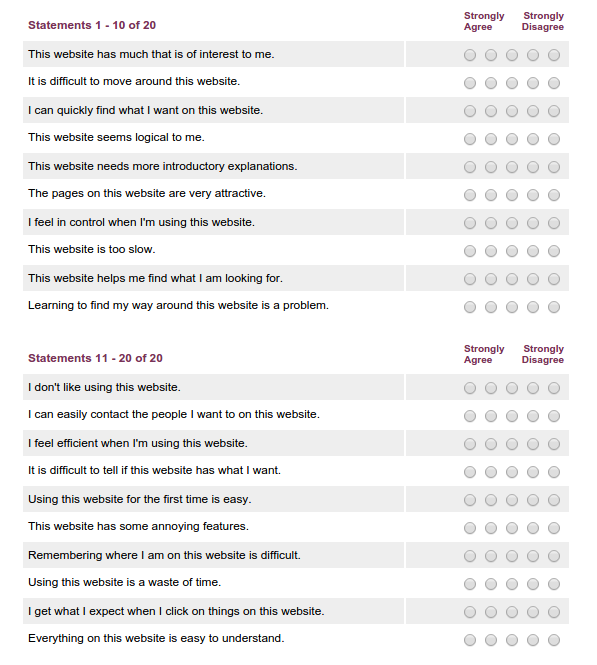
\includegraphics[scale=0.67]{editaveis/figuras/wammi_questions}
	\caption[Exemplo de itens do questionário WAMMI]{Exemplo de itens do questionário WAMMI. \footnotemark}
	\label{wammi_questions}
      \end{figure}
      
      As questões do WAMMI permitem analisar cinco fatores de usabilidade, Atratividade, Controlabilidade, Eficiência, Utilidade
      e Capacidade de aprendizado por meio de um padrão de resposta gradativo de cinco escalas que varia de “Concordo fortemente”
      a “Discordo fortemente”.
      \footnotetext{Disponível em: <http://www.wammi.com/samples/>.}
      
      Os serviços de análise das questões fornecidos pelo WAMMI são únicos, devido a todo arcabouço matemático e científico
      envolvido na sua construção, e, apesar do WAMMI ser voltado para \textit{websites}, para poder utilizá-lo no projeto, as perguntas
      podem ser adaptadas ao contexto do projeto para fornecer uma avaliação das metas de usabilidade Atratividade,
      Controlabilidade, Eficiência, Utilidade e Capacidade de aprendizado da aplicação.
    
    \subsection{\textit{Questionnaire for User Interface Satisfaction} - QUIS}
      
      \nocite{quis}
      O QUIS é um tipo de questionário que avalia a satisfação do usuário em relação a usabilidade do produto quanto à sua
      padronização, a fim de obter informações de forma precisa em relação a reação dos usuários aos seus novos produtos. 
      
      O pacote QUIS é composto por questões que podem ser avaliadas em uma escala de 0 a 9 e este pacote é possui um documento
      de texto composto por todas as seções do questionário que podem ser editadas de acordo com a necessidade de avaliação do 
      \textit{software}, possui uma versão única do questionário aplicado em HTML e possui também uma seleção dos trabalhos relevantes
      que detalham a validação do QUIS e alguns de seus usos. 
      
      O aplicativo \textit{MyPush} seguirá alguns padrões de interface para atender melhor a satisfação dos usuários na utilização do
      aplicativo. Esse tipo de questionário pode ser aplicado para garantir que a usabilidade seja levada em conta no processo de
      criação de interfaces do aplicativo e para verificar se o aplicativo está de conforme com as expectativas do usuário, 
      avaliando o seu grau de satisfação em relação as funcionalidades do \textit{MyPush}.
      
    \subsection{\textit{ErgoList}}
    
      O questionário ErgoList é um serviço disponibilizado via internet composto de uma base de conhecimento em ergonomia,
      que inspeciona, através de um \textit{checklist}, interfaces homem-computador. Nesse ambiente, o especialista avalia a interface 
      de uma aplicação usando o \textit{checklist} disponibilizado pelo LabIUtil. Tem uma base de questões bastante completa, cobrindo
      vários aspectos da usabilidade do \textit{software}. Por ser um \textit{checklist}, deve ser usado por um especialista com conhecimento em
      ergonomia (ERGOLIST, 2008).
      
      Este questionário leva em consideração os dezoito critérios ergonômicos de Bastien e Scapin (1993). São dezoito \textit{checklists}
      disponíveis no Ergolist, para cada um desses critérios que determina a ergonomia de uma interface homem-computador,
      totalizando 194 questões.
      
      O Ergolist é um questionário bem completo de tal modo que possui uma excelente precisão quando usado por um especialista,
      sendo muito útil para a medição.	

      Como o \textit{MyPush} é um aplicativo que pretende seguir os padrões de interface ditados pela indústria, é de vital
      importância para o seu desenvolvimento que estudos rígidos como o ErgoList sejam aplicados para que possa manter o 
      padrão desejado e o mesmo não fique aquém do esperado.
    
    \subsection{\textit{After Scenario Questionnaire} - ASQ}
    
      O questionário ASQ é um questionário feito para ser usado, como o próprio nome diz, imediatamente após cada cenário de uso
      completo, que permite avaliar a satisfação do usuário durante a participação de um estudo de usabilidade baseado em cenários,
      onde um cenário é um conjunto de tarefas relacionadas \cite{lewis91}.
      
      Consiste em apenas três itens que possuem padrão de resposta gradativo de sete escalas, que varia de “Concordo fortemente” 
      a “Discordo fortemente” e também conta com a opção “Não aplicável” fora da escala. A pontuação do questionário pode ser
      obtida pela média aritmética dos pontos de cada questão.
      
      \begin{figure}[h]
	\centering
	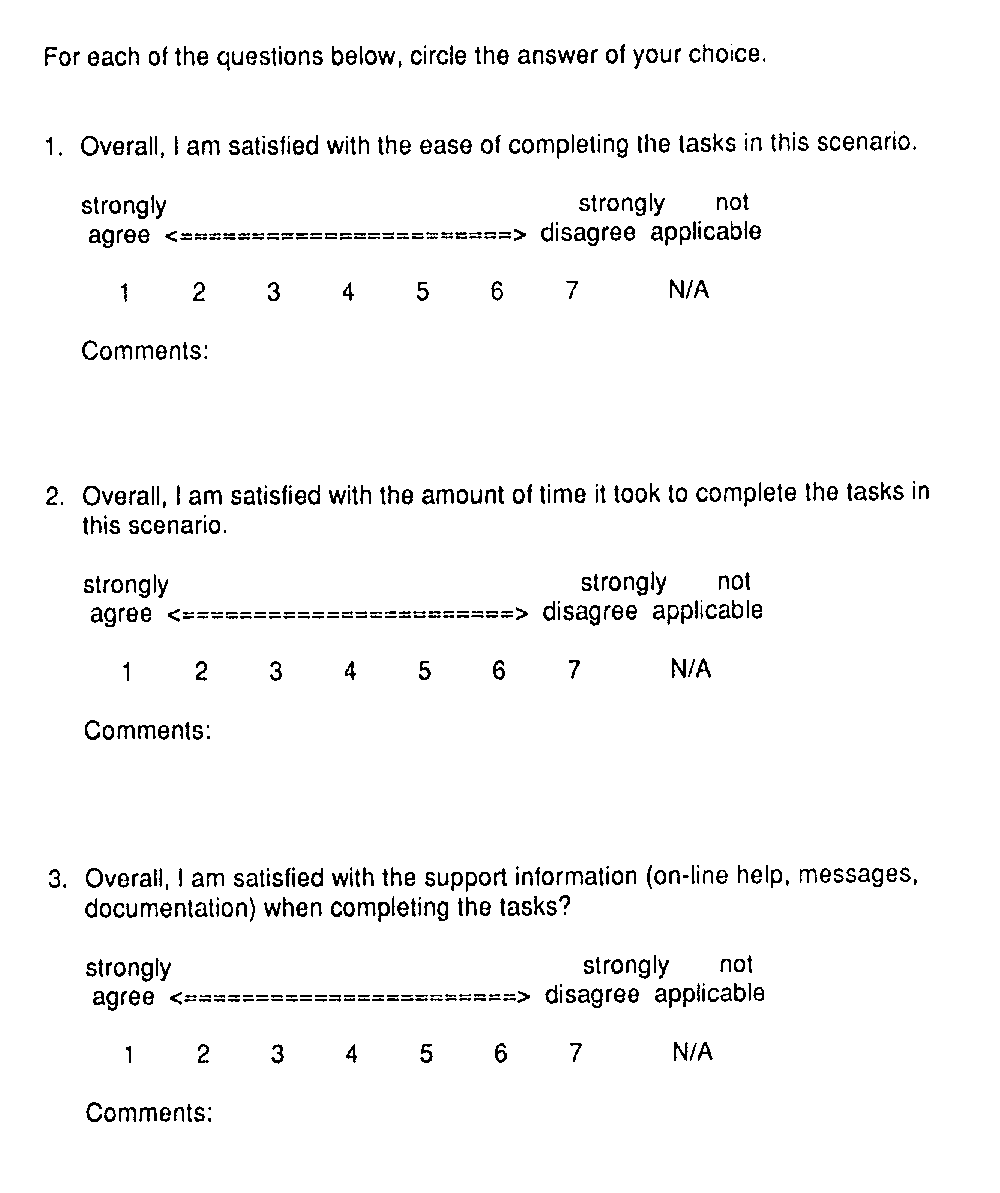
\includegraphics[scale=0.28]{editaveis/figuras/asq_questions}
	\caption[Questões do questionário ASQ]{Questões do questionário ASQ. Fonte: \cite{lewis91}.}
	\label{asq_questions}
      \end{figure}
      
      Os aspectos abordados nos itens do ASQ são: facilidade de completar as tarefas, tempo necessário para completar as tarefas 
      e satisfação com informações de suporte durante as tarefas, que possibilita visualizar a percepção do usuário a respeito da
      usabilidade do sistema \cite{lewis91}. A Figura ~\ref{asq_questions} mostra as três questões do ASQ.
      
      O questionário ASQ mostra se um recurso de avaliação rápido e eficaz para avaliar imediatamente a satisfação do usuário
      frente a um cenário de uso, evidenciando sua passividade de uso no projeto.
    
    \subsection{\textit{Post Study System Usability Questionnaire} - PSSUQ}
      
      O questionário PSSUQ é um instrumento que também permite avaliar a satisfação percebida pelo usuário ao utilizar um
      sistema \cite{lewis02}. Diferentemente do ASQ, o PSSUQ deve ser aplicado após completado um conjunto definido de cenários,
      para avaliar de forma generalizada o sistema (um conjunto de cenários).
      
      Assim como o ASQ, o PSSUQ também possui um padrão gradativo de resposta de sete escalas que varia de “Concordo fortemente”
      a “Discordo fortemente” e possui a opção “Não aplicável” fora da escala, porém conta com dezenove itens para a avaliação,
      onde cada item tem a possibilidade de receber um comentário do usuário. Os itens do PSSUQ (vide Figura ~\ref{pssuq_questions})
      permite avaliar o sistema em quatro aspectos, fornecendo medidas para cada um deles. São eles:
      
      \begin{itemize}
       \item \textit{SysUse} - Avalia a usabilidade do sistema (\textit{System Usefulness}).
	  \subitem Questões 1-8;
      
       \item \textit{InfoQual} - Avalia a qualidade da informação fornecida pelo sistema. (\textit{Information Quality})
	  \subitem Questões 9-15;
	  
       \item \textit{InterQual} - Avalia a qualidade da interface do sistema (\textit{Interface Quality}).
	  \subitem Questões 16-18;
       
       \item \textit{Overall} - Avalia a satisfação geral do usuário com o sistema.
	  \subitem Questões 1-19.

      \end{itemize}
      
      Para obter a pontuação de qualquer área, basta calcular a média aritmética das pontuações das questões relacionadas à área.
      
      
      Um ponto interessante deste questionário é que, devido a utilização de técnicas psicométricas, a não observância de
      algumas questões não impacta significativamente no resultado obtido, ou seja, um questionário incompleto possui, 
      tecnicamente, a mesma confiabilidade de um questionário completo \cite{lewis02}. Outro ponto interessante é que o
      resultado do PSSUQ não possui variações significativas em detrimento ao sexo do usuário \cite{lewis02}.
      
      \begin{figure}[!htpb]
	\centering
	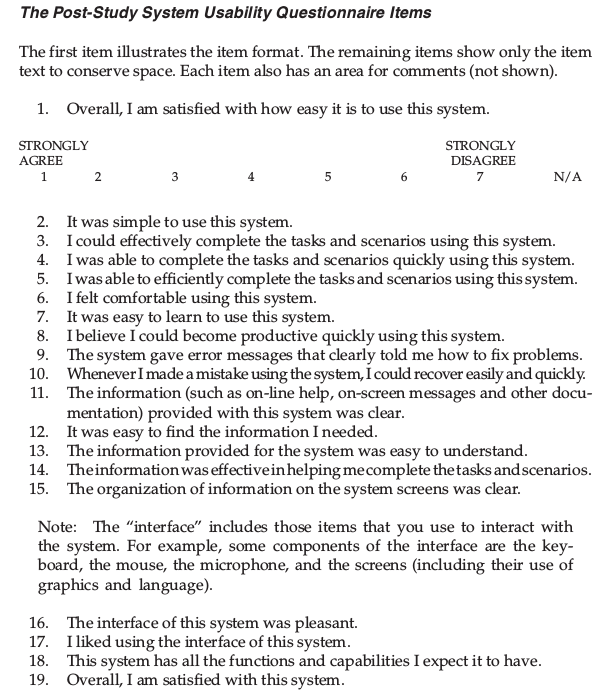
\includegraphics[scale=0.7]{editaveis/figuras/pssuq_questions}
	\caption[Questões do questionário PSSUQ]{Questões do questionário PSSUQ. Fonte: \cite{lewis02}.}
	\label{pssuq_questions}
      \end{figure}
      
      Com o que foi exposto, percebe-se que o PSSUQ é um questionário poderoso que permite uma avaliação confiável da
      satisfação do usuário em relação ao sistema. Como o PSSUQ deve ser utilizado após um conjunto de cenários ter sido
      completado, o seu uso concomitante com o ASQ se mostra uma prática promissora para a avaliação, pois, enquanto o ASQ
      retorna um feedback a cada c
      enário realizado, o PSSUQ permite um feedback geral do sistema que está sendo analisado.
    
    \subsection{Questionários escolhidos}

      A princípio foram escolhidos os questionários ASQ, para avaliação após cada cenário de uso, e PSSUQ, para a avaliação
      do conjunto de todos os cenários, que diz respeito ao produto final.
    
    \vfill
    
    \pagebreak
    \section{Planejamento das avaliações feitas no projeto}
      
      \subsection{Para o protótipo de papel}
      
	Essa seção apresenta o planejamento feito para as iterações de avaliação do protótipo de papel.
      
	\subsubsection{Iteração 1}
	  
	  \begin{itemize}
	   \item \textbf{Objetivo da avaliação}
	      
	      \subitem Essa iteração de avaliação tem por objetivo primário levantar requisitos para aplicação inicial.
	      
	      \subitem \textbf{Metas e princípios de usabilidade}\\
		Também faz parte do intuito da avaliação analisar as seguintes metas e princípios de usabilidade para o protótipo:
		
		\subsubitem - Utilidade
		\subsubitem - Eficácia
		\subsubitem - Visibilidade
		\subsubitem - \textit{Feedback}
	    
	   \item \textbf{Escopo da avaliação}
	      
	      \subitem 
		O usuário avaliará as funcionalidades existentes no protótipo de papel 
		(Programar notificação e gerenciar notificações), referentes aos requisitos funcionais iniciais levantados,
		para levantar possíveis requisitos.
	      
	   \item \textbf{Questões a se aplicar}
	      
	      \subitem Será aplicado apenas o questionário ASQ para avaliar e permitir o acompanhamento da evolução dos cenários.
	      
	   \item \textbf{Técnica de avaliação}
	      
	      \subitem 
		Serão utilizadas as técnicas de observação do usuário e de solicitação da opinião dos usuários
		sob o paradigma de avaliação \textit{'quick and dirty'}.
	      
	   \item \textbf{Questões práticas}
	      
	      \subitem Foi selecionado um grupo de 5 usuários com o perfil de uso da aplicação.
	      
	      \subitem Será necessário apenas o uso do protótipo de papel para a avaliação, não
		necessitando de outras ferramentas ou equipamentos.
	      
	   \item \textbf{Questões éticas}
	      
	      \subitem 
		Os usuários deverão assinar um termo de consentimento para participar da avaliação (em anexo).
	      
	  \end{itemize}
	
	\subsubsection{Iteração 2}
	  
	  \begin{itemize}
	  
	   \item \textbf{Objetivo da avaliação}
	      
	      \subitem Essa iteração de avaliação tem por objetivo primário levantar e estabilizar
		requisitos para aplicação inicial.
	      
	      \subitem \textbf{Metas e princípios de usabilidade}\\
		Também faz parte do intuito da avaliação analisar as seguintes metas e princípios de usabilidade para o protótipo:
		
		\subsubitem - Utilidade
		\subsubitem - Eficácia
		\subsubitem - Visibilidade
		\subsubitem - \textit{Feedback}
	    
	   \item \textbf{Escopo da avaliação}
	      
	      \subitem 
		O usuário avaliará as funcionalidades existentes no protótipo de papel 
		(Programar notificação e gerenciar notificações, com as novas mudanças do resultado da iteração 1),
		referentes aos requisitos funcionais levantados, para levantar possíveis requisitos.
	      
	   \item \textbf{Questões a se aplicar}
	      
	      \subitem Será aplicado apenas o questionário ASQ para avaliar e permitir o acompanhamento da evolução dos cenários.
	      
	   \item \textbf{Técnica de avaliação}
	      
	      \subitem 
		Serão utilizadas as técnicas de observação do usuário e de solicitação da opinião dos usuários
		sob o paradigma de avaliação \textit{'quick and dirty'}.
	      
	   \item \textbf{Questões práticas}
	      
	      \subitem Foi selecionado um grupo de 5 usuários com o perfil de uso da aplicação.
	      
	      \subitem Serão necessários o protótipo de papel e uma câmera para a realização da avaliação.
	      
	   \item \textbf{Questões éticas}
	      
	      \subitem 
		Os usuários deverão assinar um termo de consentimento para participar da avaliação (em anexo).
	   
	  \end{itemize}
      
      \subsection{Para o protótipo de alta fidelidade}
	
	Essa seção apresenta o planejamento feito para as iterações de avaliação do protótipo de alta fidelidade, feito na
	ferramenta \textit{Just in Mind}.
	
	\subsubsection{Iteração 1}
	
	  \begin{itemize}
	   \item \textbf{Objetivo da avaliação}
	      
	      \subitem Essa iteração de avaliação tem por objetivo primário avaliar os quesitos de usabilidade do protótipo.
	      
	      \subitem \textbf{Metas e princípios de usabilidade}\\
		O intuito da avaliação é analisar as seguintes metas e princípios de usabilidade para o protótipo, além das
		heurísticas de usabilidade de Nielsen:
		
		\subsubitem - Utilidade
		\subsubitem - Eficácia
		\subsubitem - Eficiência
		\subsubitem - Visibilidade
		\subsubitem - \textit{Feedback}
	    
	   \item \textbf{Escopo da avaliação}
	      
	      \subitem \textbf{Cenários de avaliação com as tarefas a serem realizados pelos usuários}:
		
		\begin{itemize}
		  \item Cenário 1 - Criar uma nova notificação para determinado tema, sem adicionar um comentário.
		    
% 		    \subitem \textbf{Caminho esperado:}
% 		      \subsubitem
		    
		  \item Cenário 2 - Editar a hora da notificação criada e adicionar um comentário à notificação.
		    
% 		    \subitem \textbf{Caminho esperado:}
% 		      \subsubitem
		    
		  \item Cenário 3 - Apagar a notificação criada.
		    
% 		    \subitem \textbf{Caminho esperado:}
% 		      \subsubitem
		  
		\end{itemize}

	   \item \textbf{Questões a se aplicar}
	      
	      \subitem Será aplicado os questionários ASQ e o PSSUQ para avaliar e permitir o acompanhamento
		da evolução dos cenários e do sistema, no geral.
	      
	   \item \textbf{Técnica de avaliação}
	      
	      \subitem 
		Serão utilizadas as técnicas de observação do usuário e de solicitação da opinião dos usuários
		sob o paradigma de avaliação de teste de usabilidade.
	      
	   \item \textbf{Questões práticas}
	      
	      \subitem Foi selecionado um grupo de 5 usuários com o perfil de uso da aplicação.
	      
	      \subitem Será necessário o uso do protótipo em um \textit{smartphone} ou em um computador, e uma câmera para 
	      a recordação da avaliação.
	      
	   \item \textbf{Questões éticas}
	      
	      \subitem 
		Os usuários deverão assinar um termo de consentimento para participar da avaliação (em anexo).
	      
	  \end{itemize}
	
	